\documentclass[a4paper,12pt]{article}
%\documentclass[a4paper,10pt]{scrartcl}

\usepackage[utf8x]{inputenc}
\usepackage{amsfonts}
\usepackage{amsmath,esint}
\usepackage{graphicx}
\usepackage{pdfpages}
\usepackage{sansmath}
\usepackage{hyperref}
\usepackage{natbib}
\usepackage{caption}
\usepackage{tikz}
\usepackage{algorithm}
\usepackage[noend]{algpseudocode}

\usepackage{titling}
\setlength{\droptitle}{-5em}   % This is your set screw
\renewcommand{\familydefault}{\sfdefault}


% ------------------------------------------------------------------
\newcommand{\permittivity}{\boldsymbol{\varepsilon}}
\newcommand{\conductivity}{\boldsymbol{\sigma}}
\newcommand{\permittivityperturb}{\hat{\boldsymbol{\varepsilon}}}
\newcommand{\conductivityperturb}{\hat{\boldsymbol{\sigma}}}
\newcommand{\permittivitysolu}{\boldsymbol{\varepsilon}_*}
\newcommand{\conductivitysolu}{\boldsymbol{\sigma}_*}
% ------------------------------------------------------------------
\newcommand{\umat}{\mathbf{u}}
\newcommand{\Lw}{\mathbf{L}_w}
\newcommand{\sw}{\mathbf{s}_w}
\newcommand{\dw}{\mathbf{d}_w}
\newcommand{\dwo}{\mathbf{d}^o_w}
\newcommand{\dwos}{\mathbf{d}^{o,s}_w}
\newcommand{\Mw}{\mathbf{M}_w}
\newcommand{\umatdot}{\dot{\mathbf{u}}}
\newcommand{\ew}{\mathbf{e}_w}
\newcommand{\vw}{\mathbf{v}_w}
\newcommand{\gwe}{\mathbf{g}_{\varepsilon}}
\newcommand{\gws}{\mathbf{g}_{w,\sigma}}
\newcommand{\dt}{\Delta t}
\newcommand{\dx}{\Delta x}
\newcommand{\dz}{\Delta z}
\newcommand{\dsigmaw}{\dsigma_w}
\newcommand{\depsi}{\Delta\boldsymbol{\varepsilon}}
\newcommand{\stepepsi}{\alpha_\varepsilon}
\newcommand{\stepsigm}{\alpha_\sigma}
\newcommand{\kappaepsi}{\kappa_\varepsilon}
\newcommand{\kappasigm}{\kappa_{w,\sigma}}
\newcommand{\depsimomentum}{\Delta\boldsymbol{\varepsilon}_\bullet}
% ------------------------------------------------------------------
\newcommand{\electpotential}{\boldsymbol{\varphi}}
\newcommand{\Ldc}{\mathbf{L}_{dc}}
\newcommand{\sdc}{\mathbf{s}_{dc}}
\newcommand{\Sdc}{\mathbf{S}_{dc}}
\newcommand{\ddc}{\mathbf{d}_{dc}}
\newcommand{\ddco}{\mathbf{d}_{dc}^o}
\newcommand{\ddcos}{\mathbf{d}_{dc}^{o,s}}
\newcommand{\Mdc}{\mathbf{M}_{dc}}
\newcommand{\edc}{\mathbf{e}_{dc}}
\newcommand{\vdc}{\mathbf{v}_{dc}}
\newcommand{\gdc}{\mathbf{g}_{dc}}
\newcommand{\dsigmadc}{\dsigma_{dc}}
\newcommand{\stepdc}{\alpha_{dc}}
\newcommand{\dsigmmomentum}{\dsigma_{dc\,\bullet}}
% ------------------------------------------------------------------
\newcommand{\Ewe}{\Theta_{w,\varepsilon}}
\newcommand{\Ewes}{\Theta_{w,\varepsilon}^s}
\newcommand{\Ews}{\Theta_{w,\sigma}}
\newcommand{\Ewss}{\Theta_{w,\sigma}^s}
\newcommand{\Ew}{\Theta_{w}}
\newcommand{\Edcs}{\Edc^s}
\newcommand{\Edc}{\Theta_{dc}}
\newcommand{\dsigma}{\Delta\boldsymbol{\sigma}}
\newcommand{\Ewphase}{\Theta_{w,\phi}}
\newcommand{\Ewenvel}{\Theta_{w,E}}
% ------------------------------------------------------------------

\title{Empirical depth of investigation of an ER experiment}
\author{Diego Domenzain}
\date{}

\begin{document}
\maketitle

% ------------------------------------------------------
%
% ------------------------------------------------------
\section{Types of arrays}
%
%
\begin{figure}[!h]
\centering
% left low right up
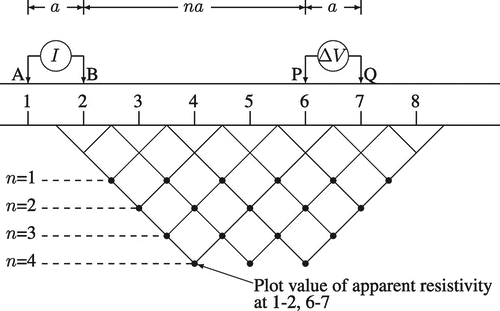
\includegraphics[width=0.4\textwidth]{../pics/dc-array-dipole-dipole-pseudosection.png}~
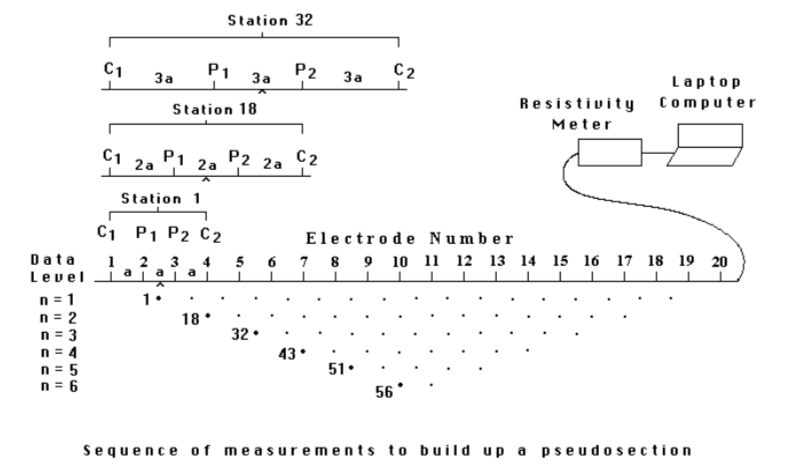
\includegraphics[width=0.4\textwidth]{../pics/wenner-pseudosection.png}\\~\\
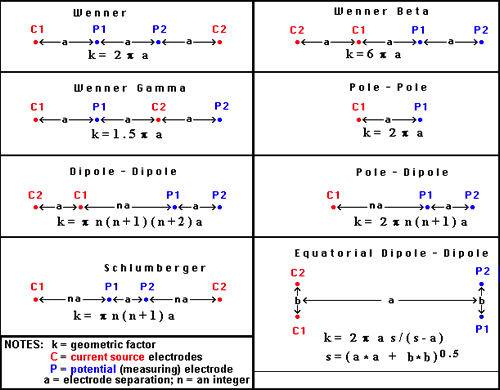
\includegraphics[width=0.6\textwidth]{../pics/dc-arrays.png}
\caption{{\bf a)} and {\bf b)}: Dipole-dipole and Wenner array configurations. {\bf c)} Other type of configurations.}
\label{fig:depth-length}
\end{figure}
% ------------------------------------------------------
%
% ------------------------------------------------------
\newpage
\section{In general}
%
%
\begin{figure}[!h]
\centering
% left low right up
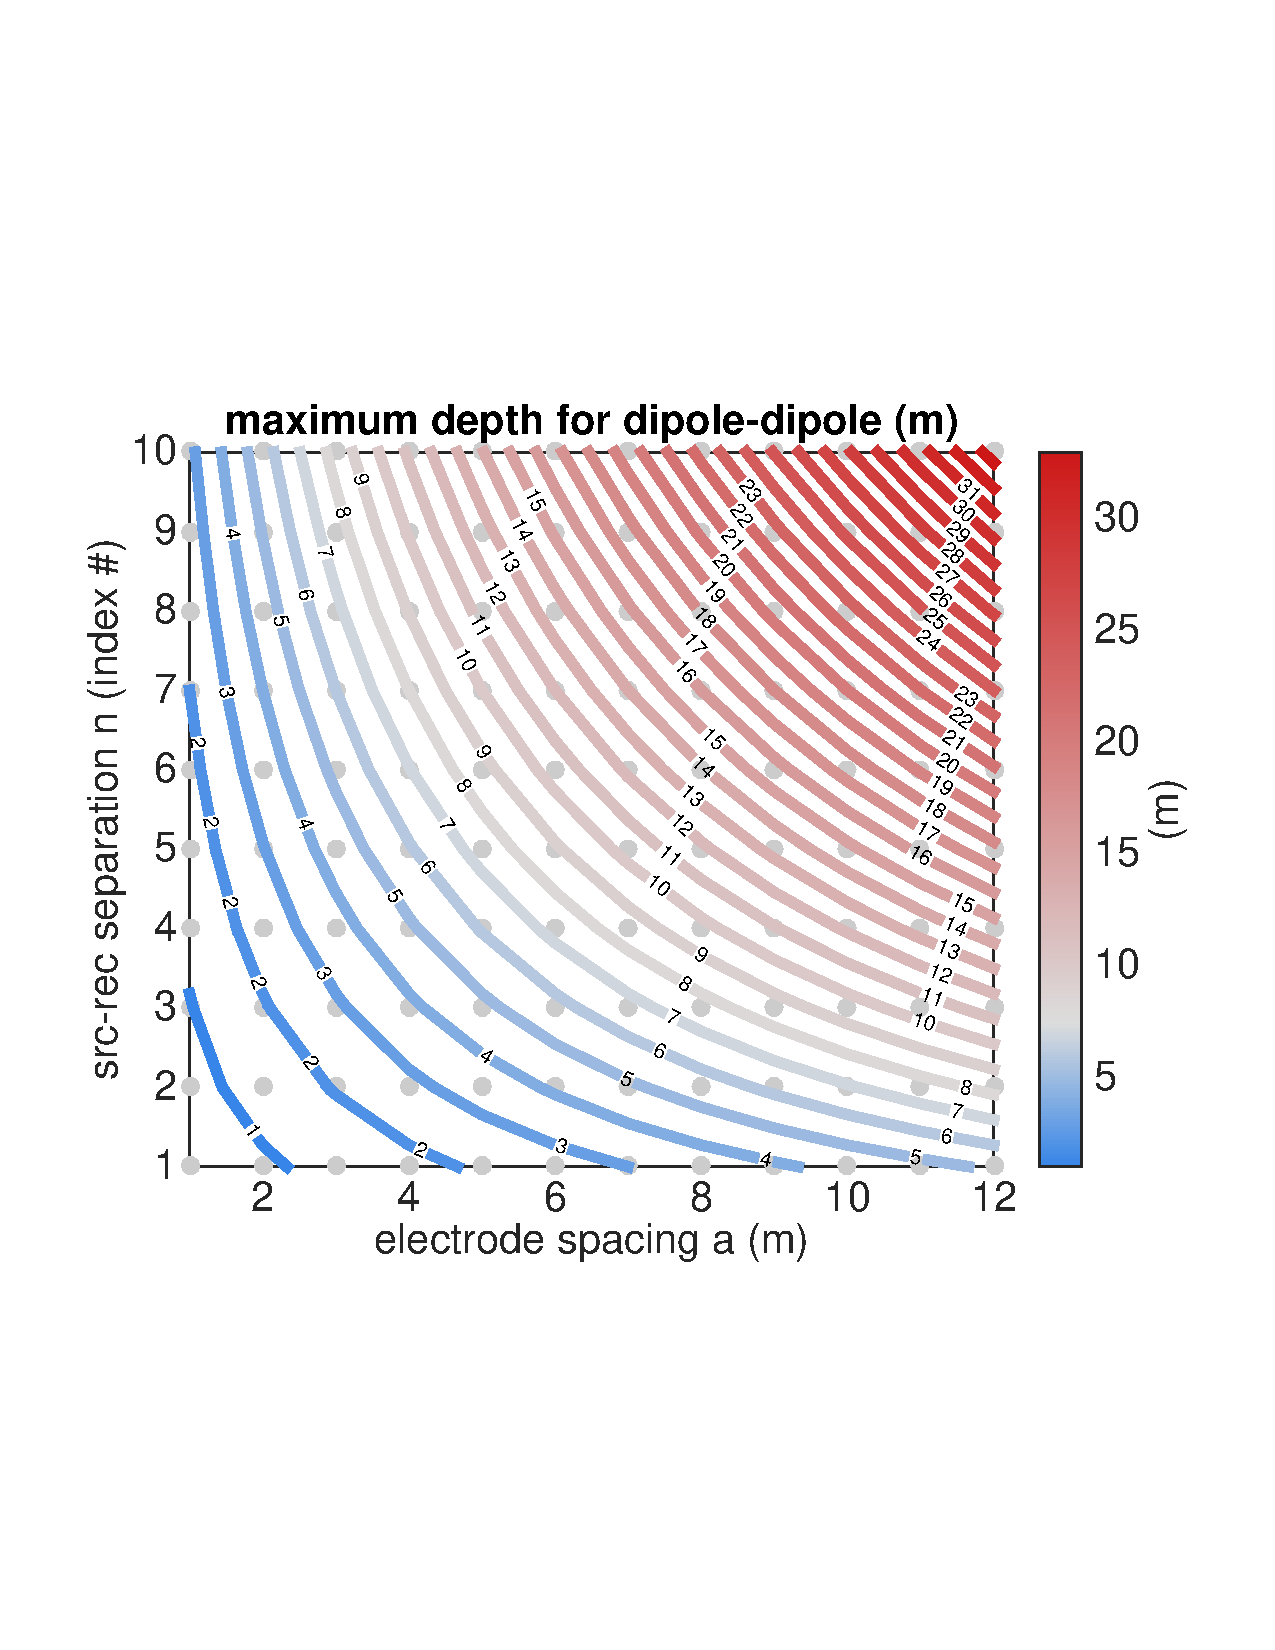
\includegraphics[trim={20 170 30 180},clip,width=0.4\textwidth]{../pics/depth-dipole.pdf}~
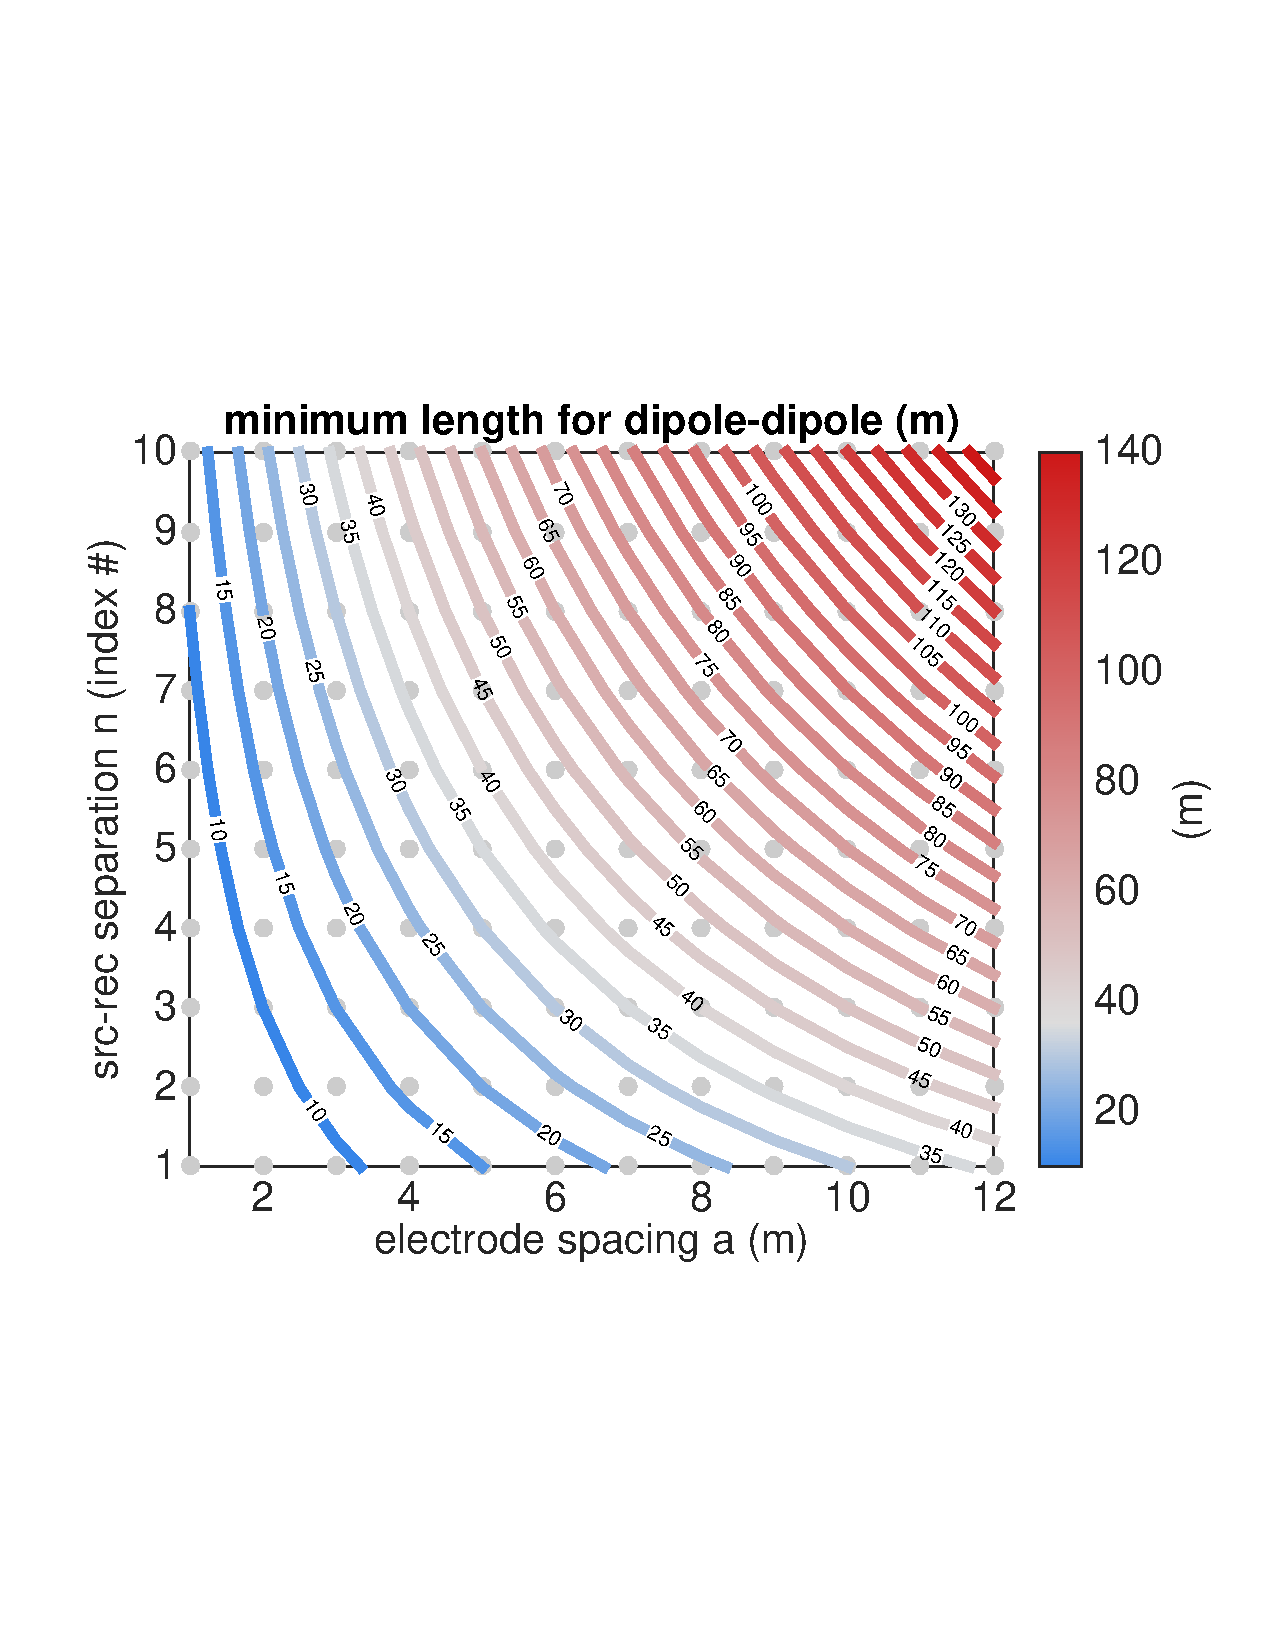
\includegraphics[trim={20 170 30 180},clip,width=0.4\textwidth]{../pics/min-length-dipole.pdf}\\~\\
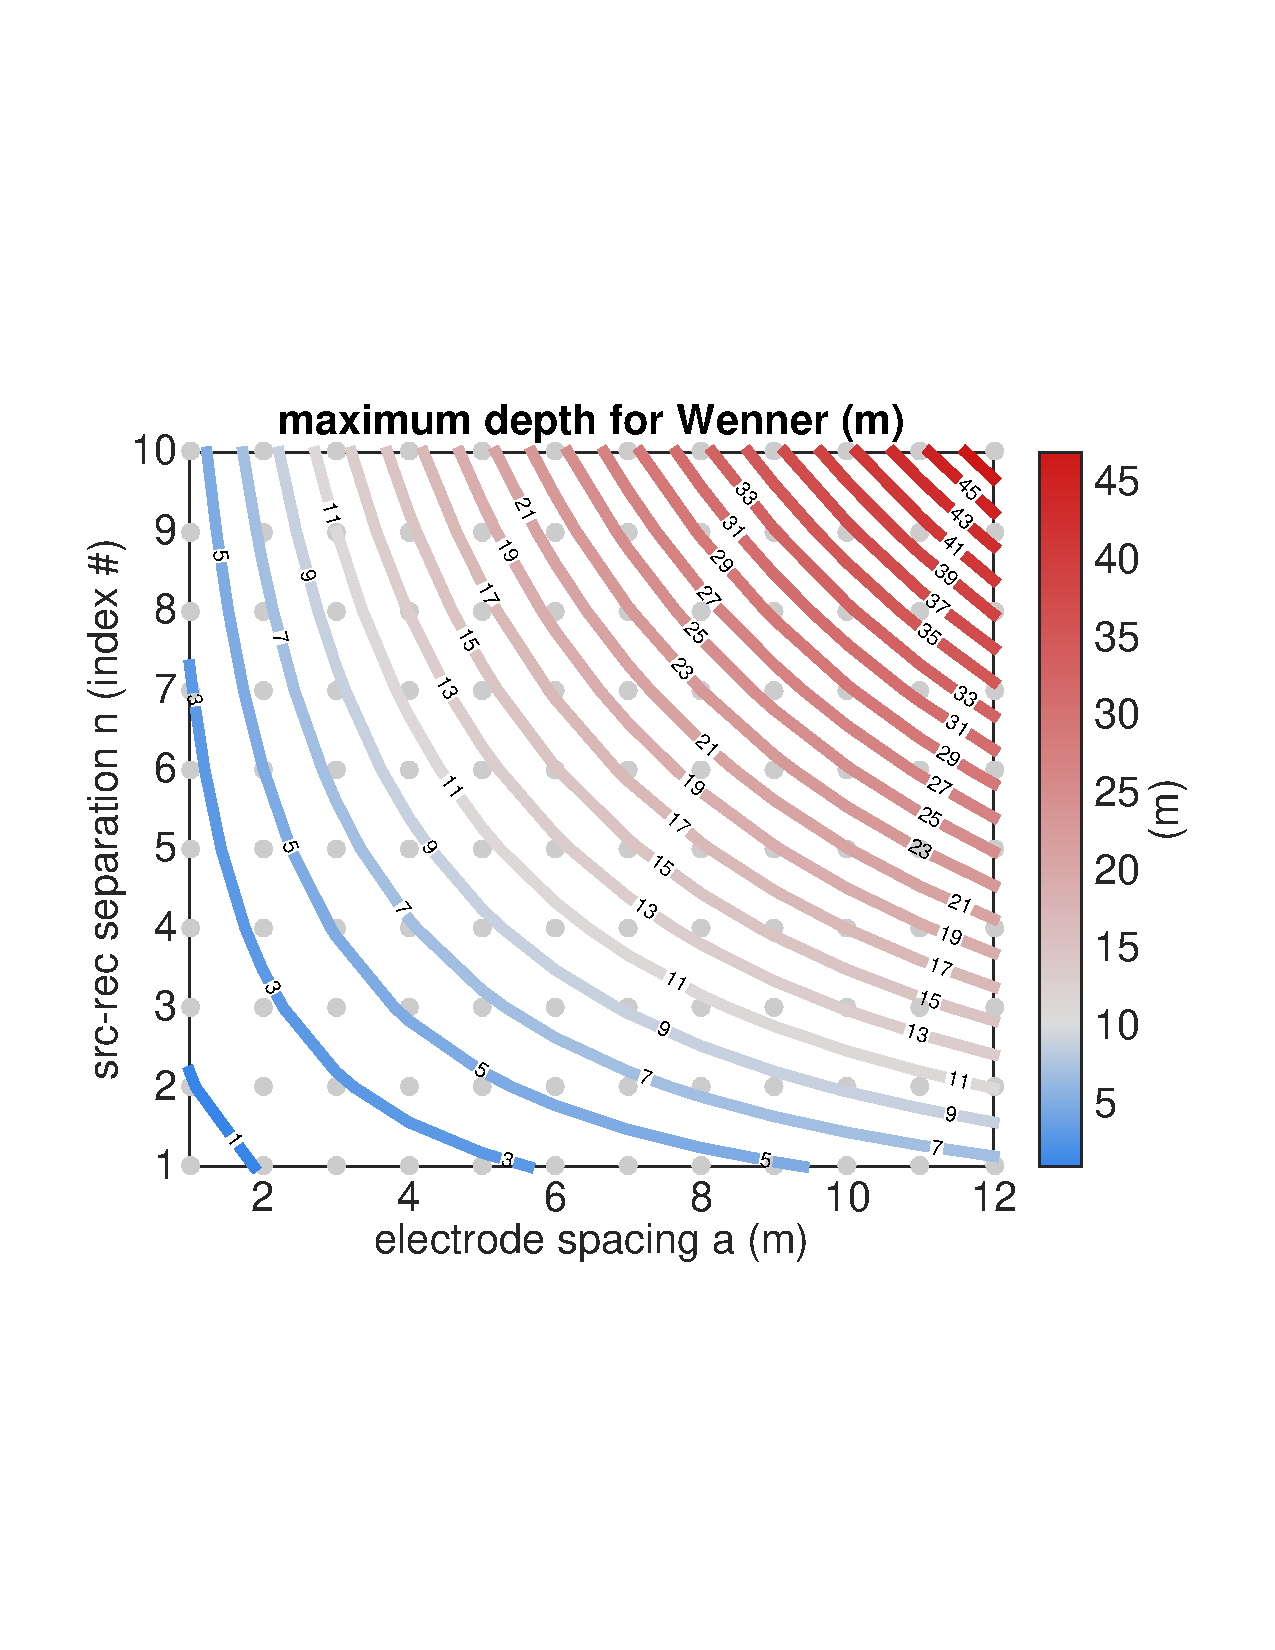
\includegraphics[trim={20 170 30 180},clip,width=0.4\textwidth]{../pics/depth-wenner.pdf}~
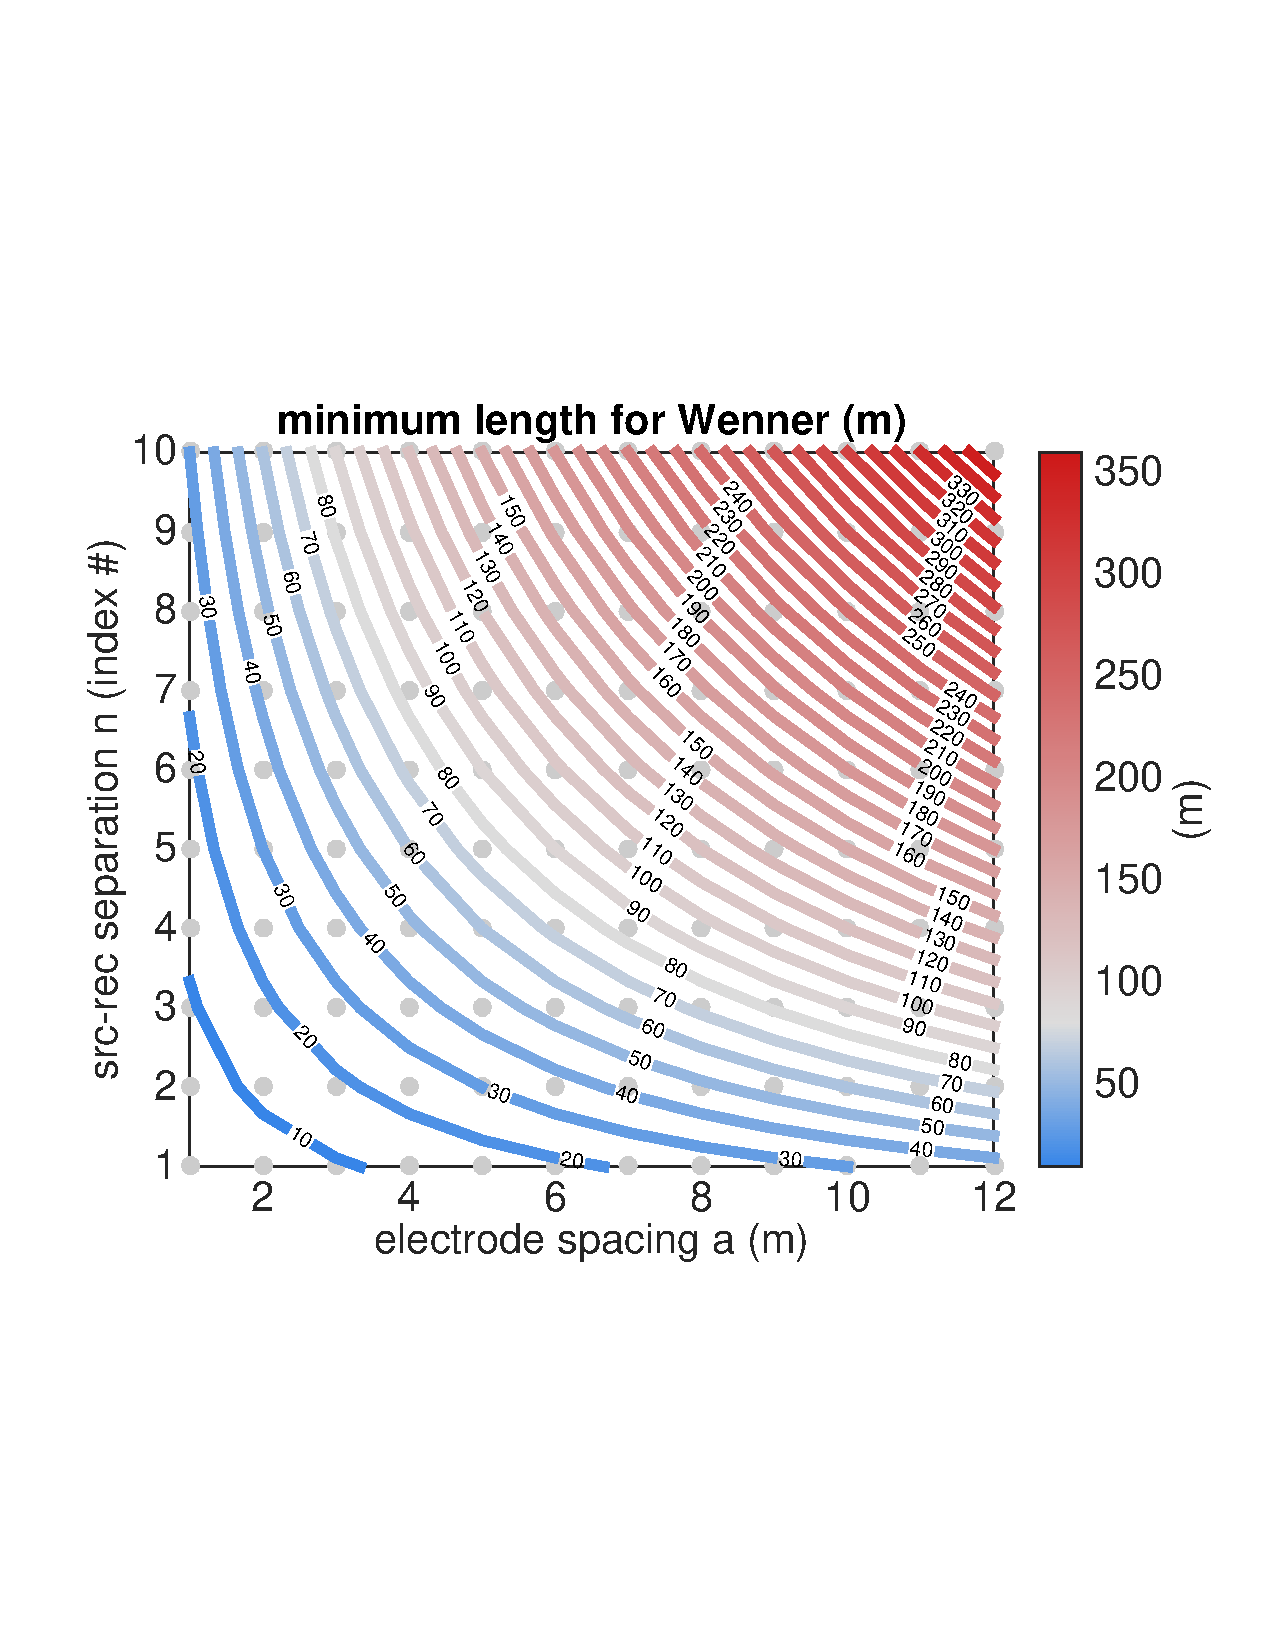
\includegraphics[trim={20 170 30 180},clip,width=0.4\textwidth]{../pics/min-length-wenner.pdf}
\caption{{\bf a)} and {\bf b)}: Maximum depth of investigation for dipole-dipole and Wenner arrays as a function of spacings $a$ and levels $n$. {\bf c)} and {\bf d)}: Minimum length of survey needed to acquire maximum depth.}
\label{fig:depth-length}
\end{figure}
%
%
% ------------------------------------------------------
%
% ------------------------------------------------------
\newpage
\section{Example for an 18m long survey}
%
%
\begin{figure}[!h]
\centering
% left low right up
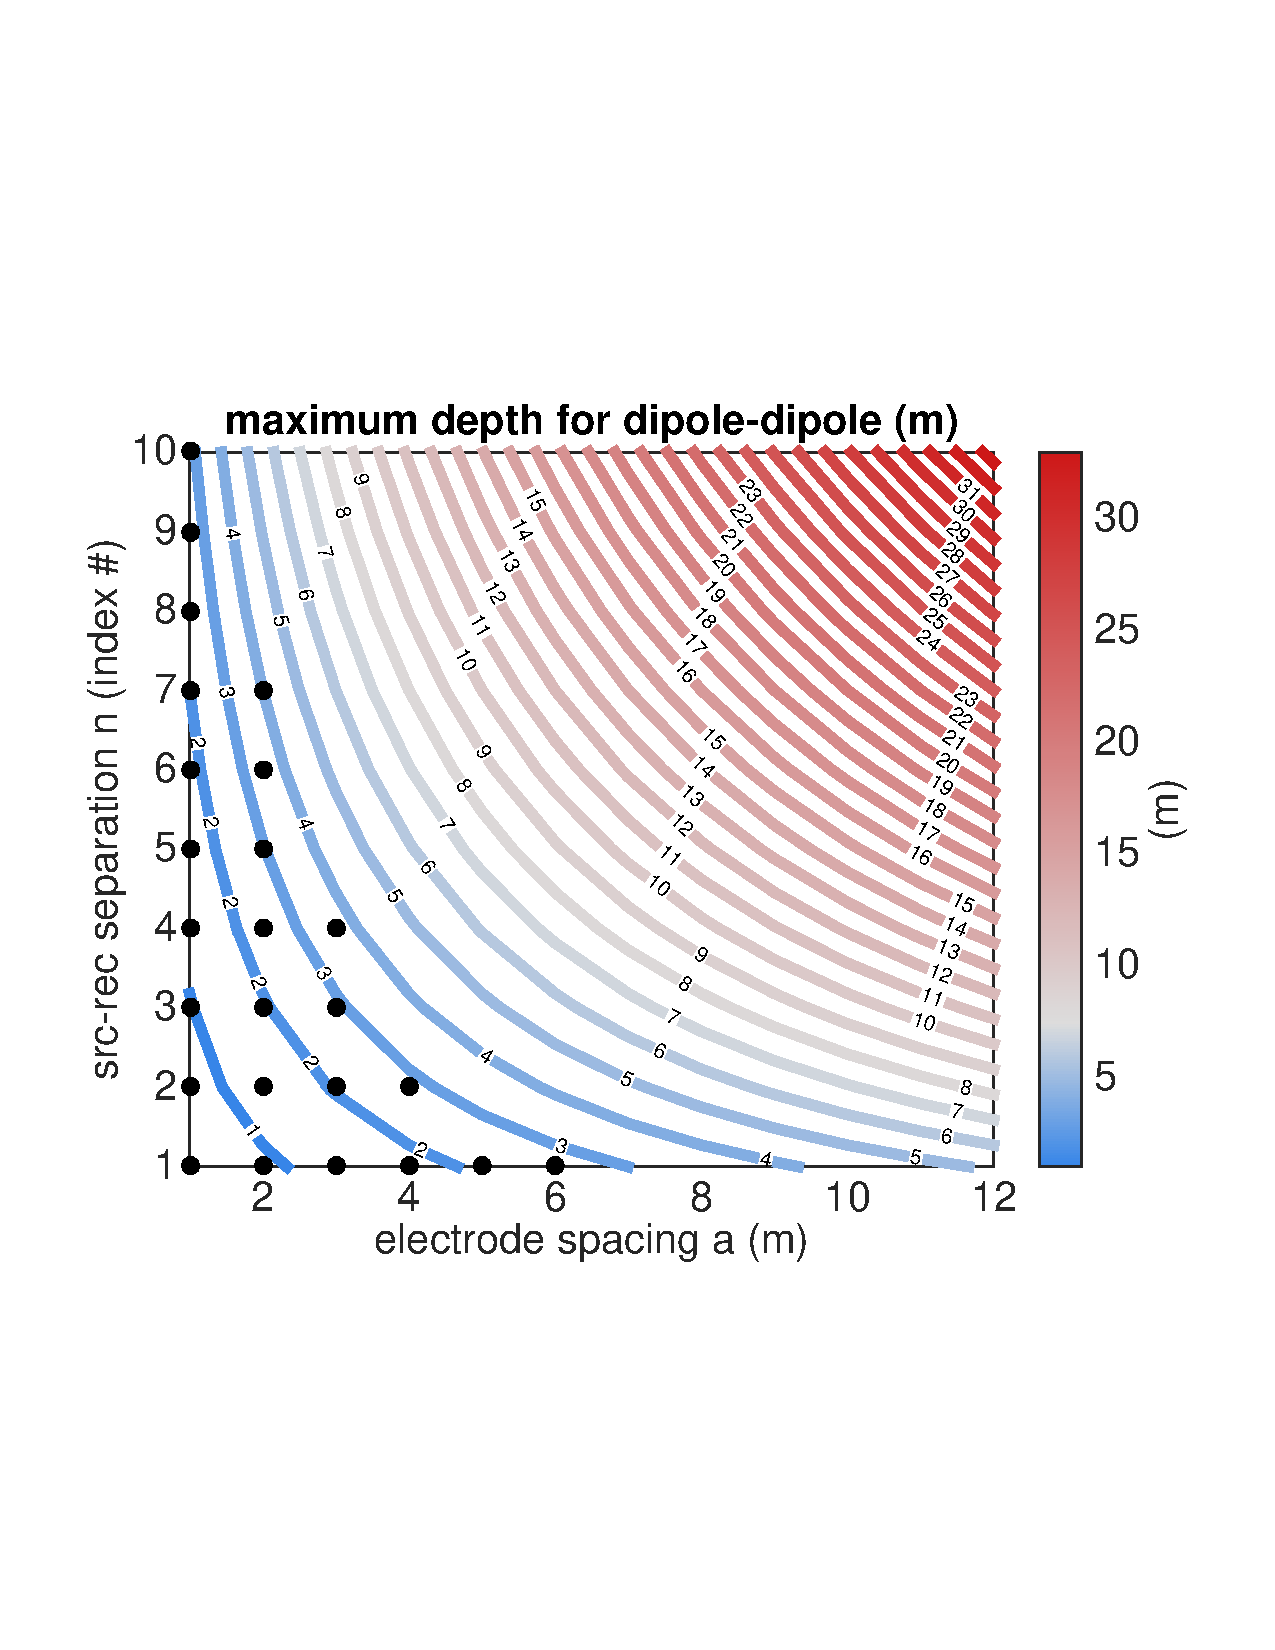
\includegraphics[trim={20 170 30 180},clip,width=0.4\textwidth]{../pics/depth-dipole-18m.pdf}~
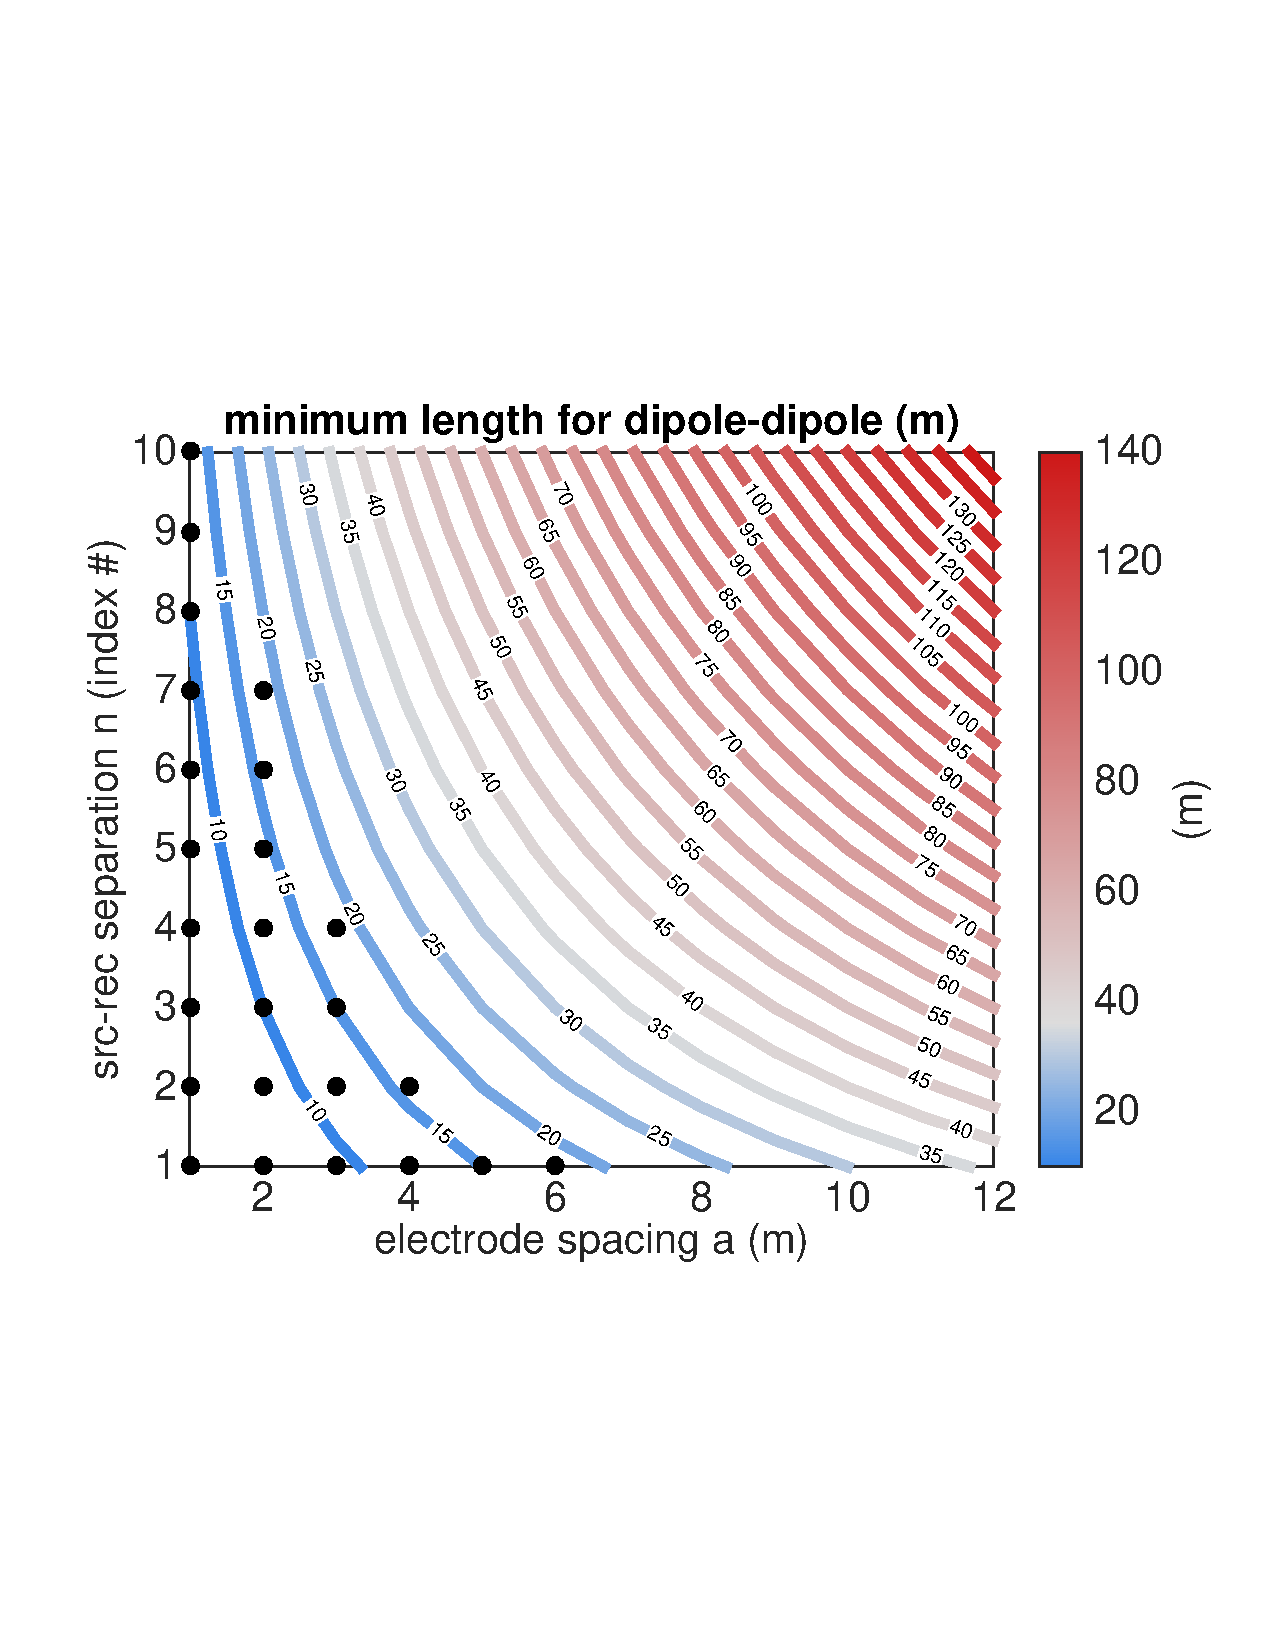
\includegraphics[trim={20 170 30 180},clip,width=0.4\textwidth]{../pics/min-length-dipole-18m.pdf}\\~\\
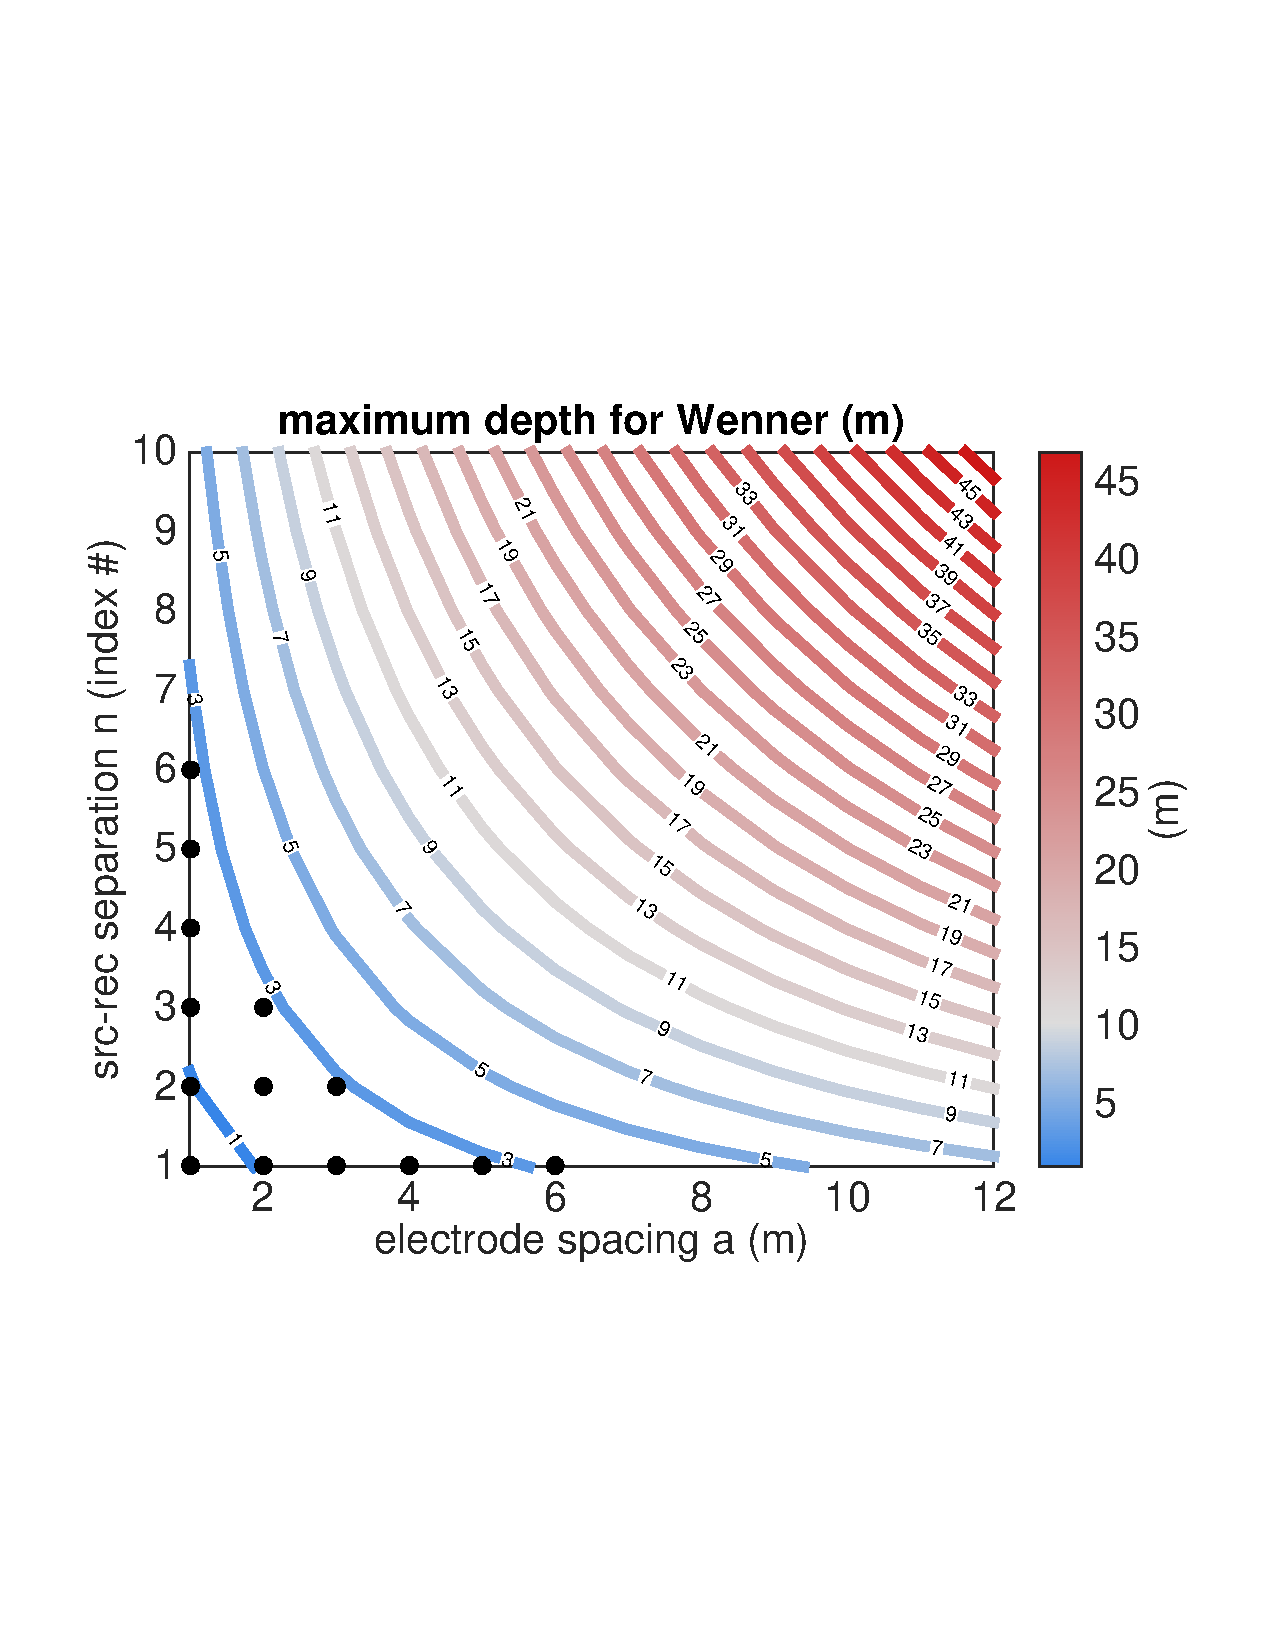
\includegraphics[trim={20 170 30 180},clip,width=0.4\textwidth]{../pics/depth-wenner-18m.pdf}~
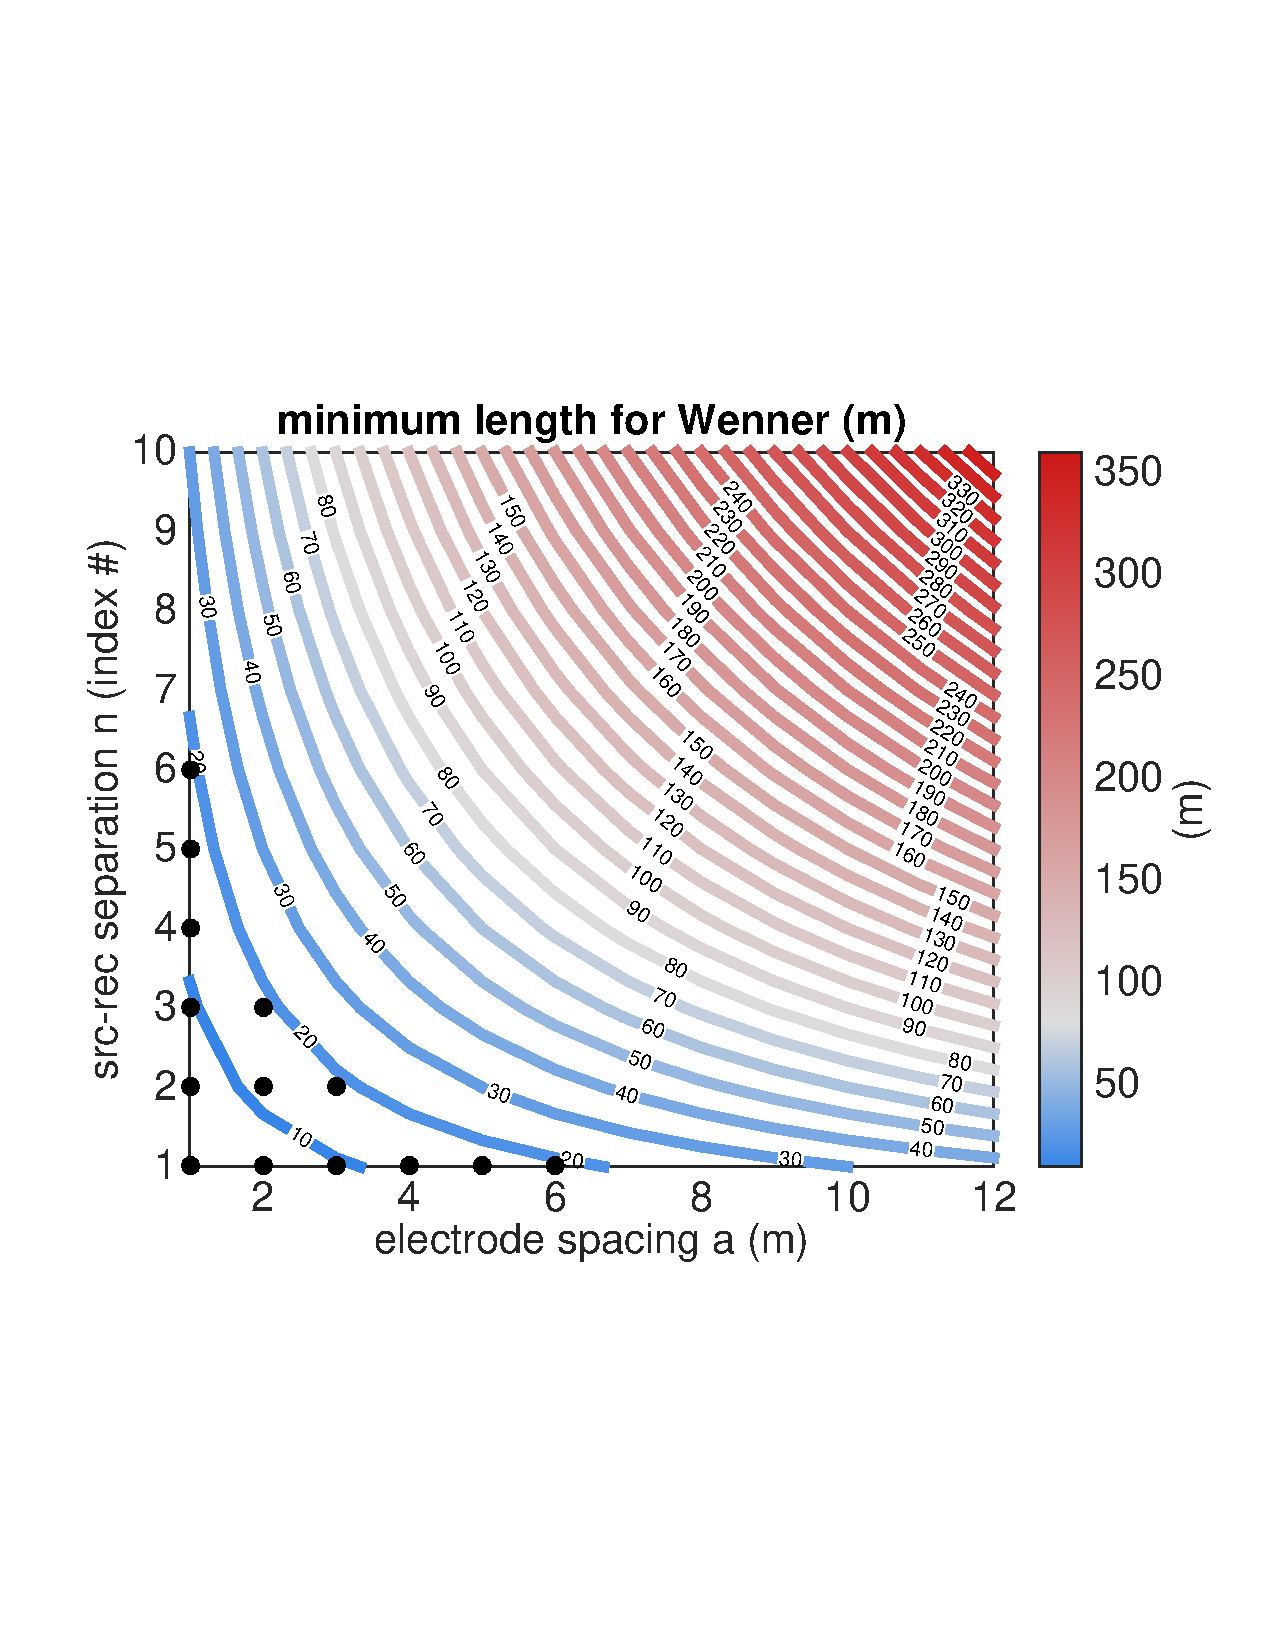
\includegraphics[trim={20 170 30 180},clip,width=0.4\textwidth]{../pics/min-length-wenner-18m.pdf}
\caption{Only black dots are taken into account when doing a survey 18m in length. {\bf a)} and {\bf b)}: Maximum depth of investigation for dipole-dipole and Wenner arrays as a function of spacings $a$ and levels $n$. {\bf c)} and {\bf d)}: Minimum length of survey needed to acquire maximum depth.}
\label{fig:depth-length}
\end{figure}
%
%
\iffalse
\begin{figure}[!h]
\centering
% left low right up
\includegraphics[width=\textwidth]{pics/pics/crop/pdfs/aw-adc-Ew-Edc.png}
\caption{Normalized objective functions history over iterations for the low {\bf a)} and high {\bf c)} conductivity scenarios. Update weights history over iterations for the low {\bf b)} and high {\bf d)} conductivity scenarios}
\label{fig:aw-adc-Ew-Edc}
\end{figure}
\fi
%
%
\end{document}
